\section{Realizarea lucrarii de laborator}

\subsection{Tasks and Points}

\begin{itemize}
\item Basic Level (nota 5 || 6) : 
\begin{itemize}

    \item conecteaza-te la server folosind SSH
    \item compileaza cel putin 2 sample programs din setul HelloWolrdPrograms folosind CLI
    \item executa primul commit folosind VCS

\end{itemize}
\item Normal Level (nota 7 || 8):
\begin{itemize}

   \item initializeaza un nou repositoriu
   \item configureaza-ti VCS
   \item crearea branch-urilor (creeaza cel putin 2 branches)
   \item commit pe ambele branch-uri (cel putin 1 commit per branch)

\end{itemize}
\item Advanced Level (nota 9 || 10): 
\begin{itemize}

   \item seteaza un branch to track a remote origin pe care vei putea sa faci push (ex. Github, Bitbucket or custom server)
   \item reseteaza un branch la commit-ul anterior
   \item merge 2 branches
   \item rezolvarea conflictelor a 2 branches

\end{itemize}
\end{itemize}

\subsection{Analiza lucrarii de laborator}
Linkul la repozitoriul GITHUB:
\begin{center}
\url{https://github.com/tarakan-x/MIDPS}
\end{center}
Pentru a realiza aceasta lucrare de laborator $m-am$ inregistrat pe github.com si am instalat $git-bash$, am generat o cheie SSH si am adaugat aceasta cheie publica pe github pentru a identifica acest calculator.\\
\begin{center}
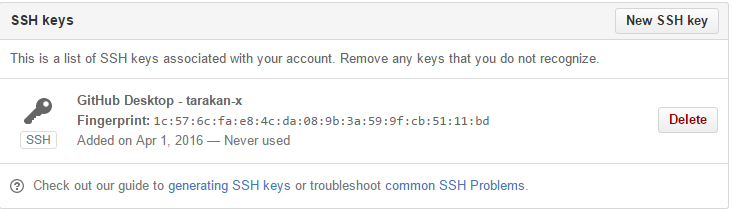
\includegraphics[scale=0.7]{images/ssh.PNG} 
\end{center}
Pentru a compila programe scrise in $C++,Java,Python$ avem nevoie de a seta directiile spre $g++,javac$ si python in fisierul bash\_profile din directoriul unde este instalat $Git-Bash$.Pentru a compila programul scris in Java utilizam javac pentru compilare si java namefile pentru a rula programul nostru,in cazul programuli $C++$ utilizam comanda $g++ $ hello.cpp -o namefille, si ./namefile pentru a rula programul si in cazul unui program scris in Python utilizam sintaxa python namefile.py pentru a rula programul.
\begin{center}
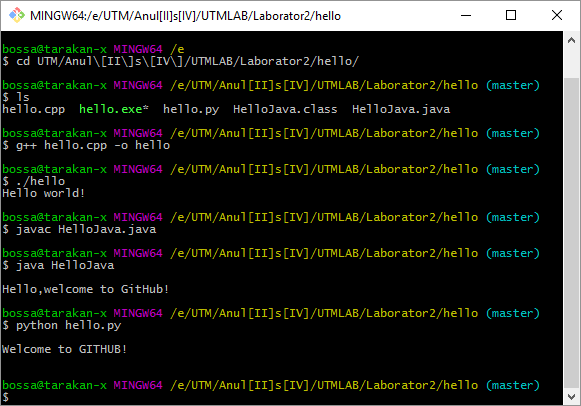
\includegraphics[scale=0.7]{images/java.png} 
\end{center}
Pentru fiecare schimbare pe care o facem pe repozitoriu putem lasa un mesaj folosind comanda git commit -m "mesaj" astfel organizam mai bine repozitoriul si putem vedea  ce schimbari au avut loc.

Am initializat un nou repozitoriu cu numele NewRep cu git init,si am configurat acest repozitoriu cu git config \--global user.name si user.email.
\begin{center}
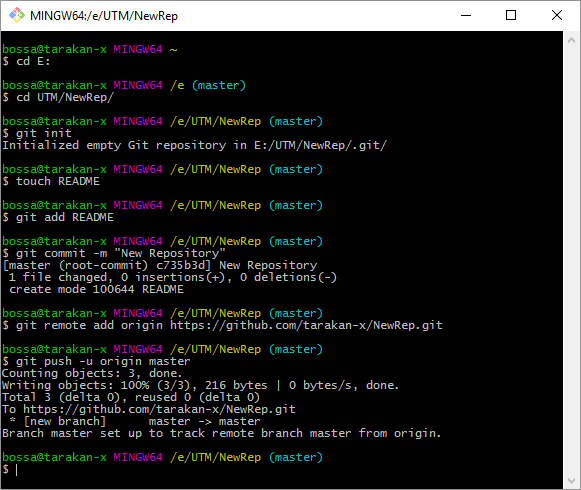
\includegraphics[scale=0.7]{images/newrep.png} 
\end{center}
Am creat doua branch-uri cu numele FIRST si SECOND folosind comanda git branch "numele".
\begin{center}
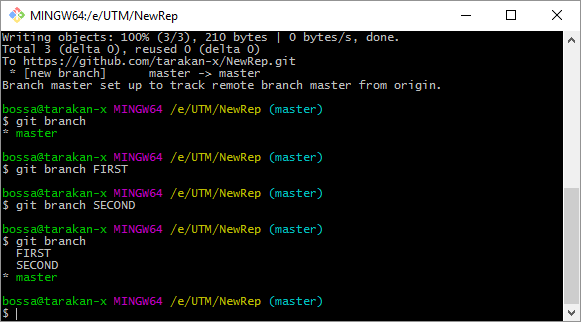
\includegraphics[scale=0.7]{images/branch.png} 
\end{center}
Am adaugat un fisier pe branch-ul FIRST.
\begin{center}
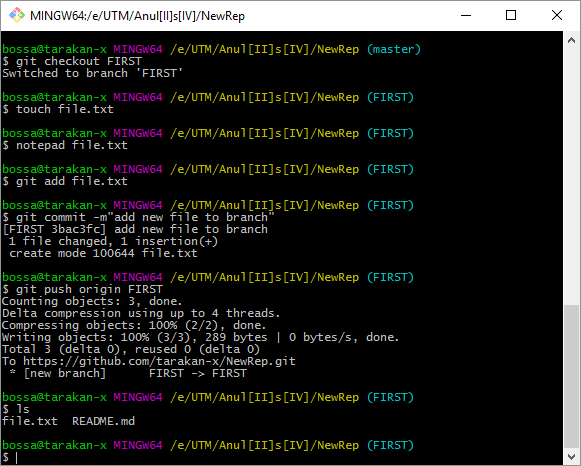
\includegraphics[scale=0.7]{images/first.png} 
\end{center}
Am adaugat si un fisier pe branch-ul SECOND.
\begin{center}
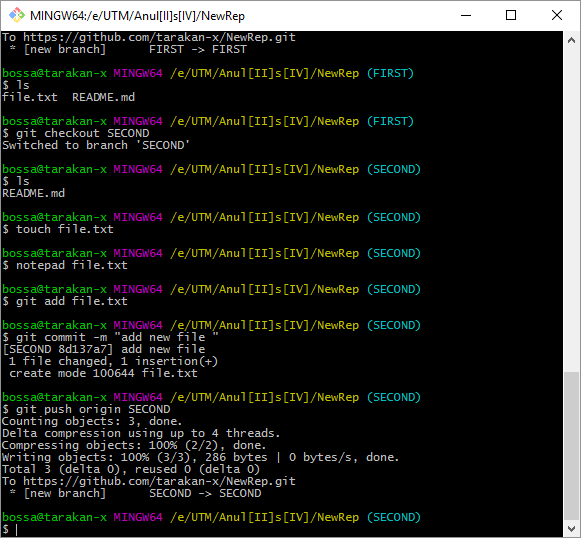
\includegraphics[scale=0.7]{images/second.png} 
\end{center}
Cind accesam github.com ca master putem accepta schimbarile de pe celelalte branch-uri astfel fisierele vor fi adaugate pe master.La fel putem lasa si un comentariu pentru acel commit.
\begin{center}
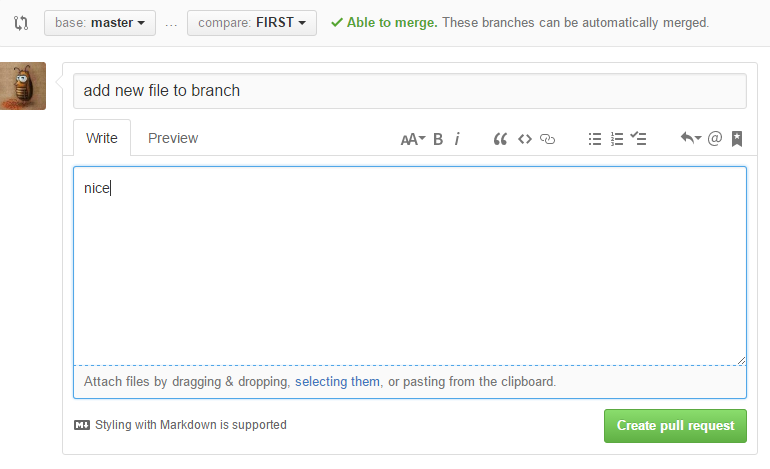
\includegraphics[scale=0.7]{images/compare.PNG}\\
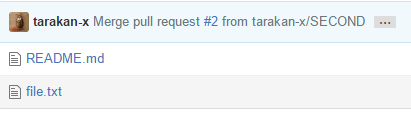
\includegraphics[scale=0.7]{images/merge.PNG} 
\end{center}
Am facut merge la branch-ul FIRST cu SECOND .
\begin{center}
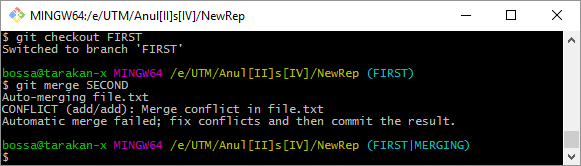
\includegraphics[scale=0.7]{images/conflict.png} 
\end{center}
In cazul cind pe un branch avem un fisier cu un continut oarecare si pe al branch acelasi fisier dar cu continut diferit atunci cind incerca sa facem merge a acestor doua branch-uri atunci primim un mesaj de conflict.Daca deschidem fisierul acolo vor fi afisate problemele care trebuie inlaturate.
\begin{center}
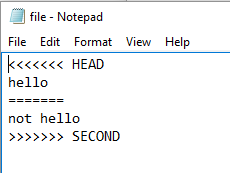
\includegraphics[scale=1]{images/fille.PNG} 
\end{center}
Pentru a rezolva aceasta problema putem modifica continutul fisierului si dupa care faceem din nou git add si commit astfel rezolvam acest conflict. 


\clearpage